\section{Υλοποίηση συστήματος \emph{RASA}}
\label{sec:rasa_impl}
Το \emph{RASA} παρέχει ένα εύχρηστο εργαλείο για την εκπαίδευση ψηφιακών βοηθών από το μηδέν με τα δεδομένα που του παρέχονται ανεξαρτήτως γλώσσας. Η εκπαίδευση γίνεται με την παροχή αρχείων τύπου \emph{YML}\footnote{\url{https://en.wikipedia.org/wiki/YAML}}. Τα βήματα που ακολουθεί ο βοηθός σε κάθε είσοδο του χρήστη μπορούν να καθοριστούν στο \emph{config.yml} αρχείο, \autoref{fig:rasax-config}. Η επιλογή της επόμενης ενέργειας του ψηφιακού βοηθού στηρίζεται σε συγκεκριμένες πολιτικές οι οποίες καθορίζονται κατά την εκπαίδευση του και περιλαμβάνονται στο ίδιο αρχείο που αναφέρθηκε προηγουμένως. Στη παρούσα υλοποίηση τα βήματα που επιλέχθηκαν ήταν:
\begin{multicols}{2}
\begin{itemize}
    \item \emph{WhitespaceTokenizer}
    \item \emph{CountVectorsFeaturizer}
    \item \emph{DIETClassifier}
    \item \emph{FallbackClassifier}
    \item \emph{DucklingEntityExtractor}
    \item \emph{MemoizationPolicy}
    \item \emph{RulePolicy}
    \item \emph{TEDPolicy}
    \item \emph{UnexpecTEDIntentPolicy}
\end{itemize}
\end{multicols}
Στο \autoref{fig:rasa-pipeline} παρουσιάζονται σχηματικά και κάθε ένα από αυτά αναλύεται στη συνέχεια.

\begin{figure}[!ht]
  \centering
  \captionsetup{justification=centering}
  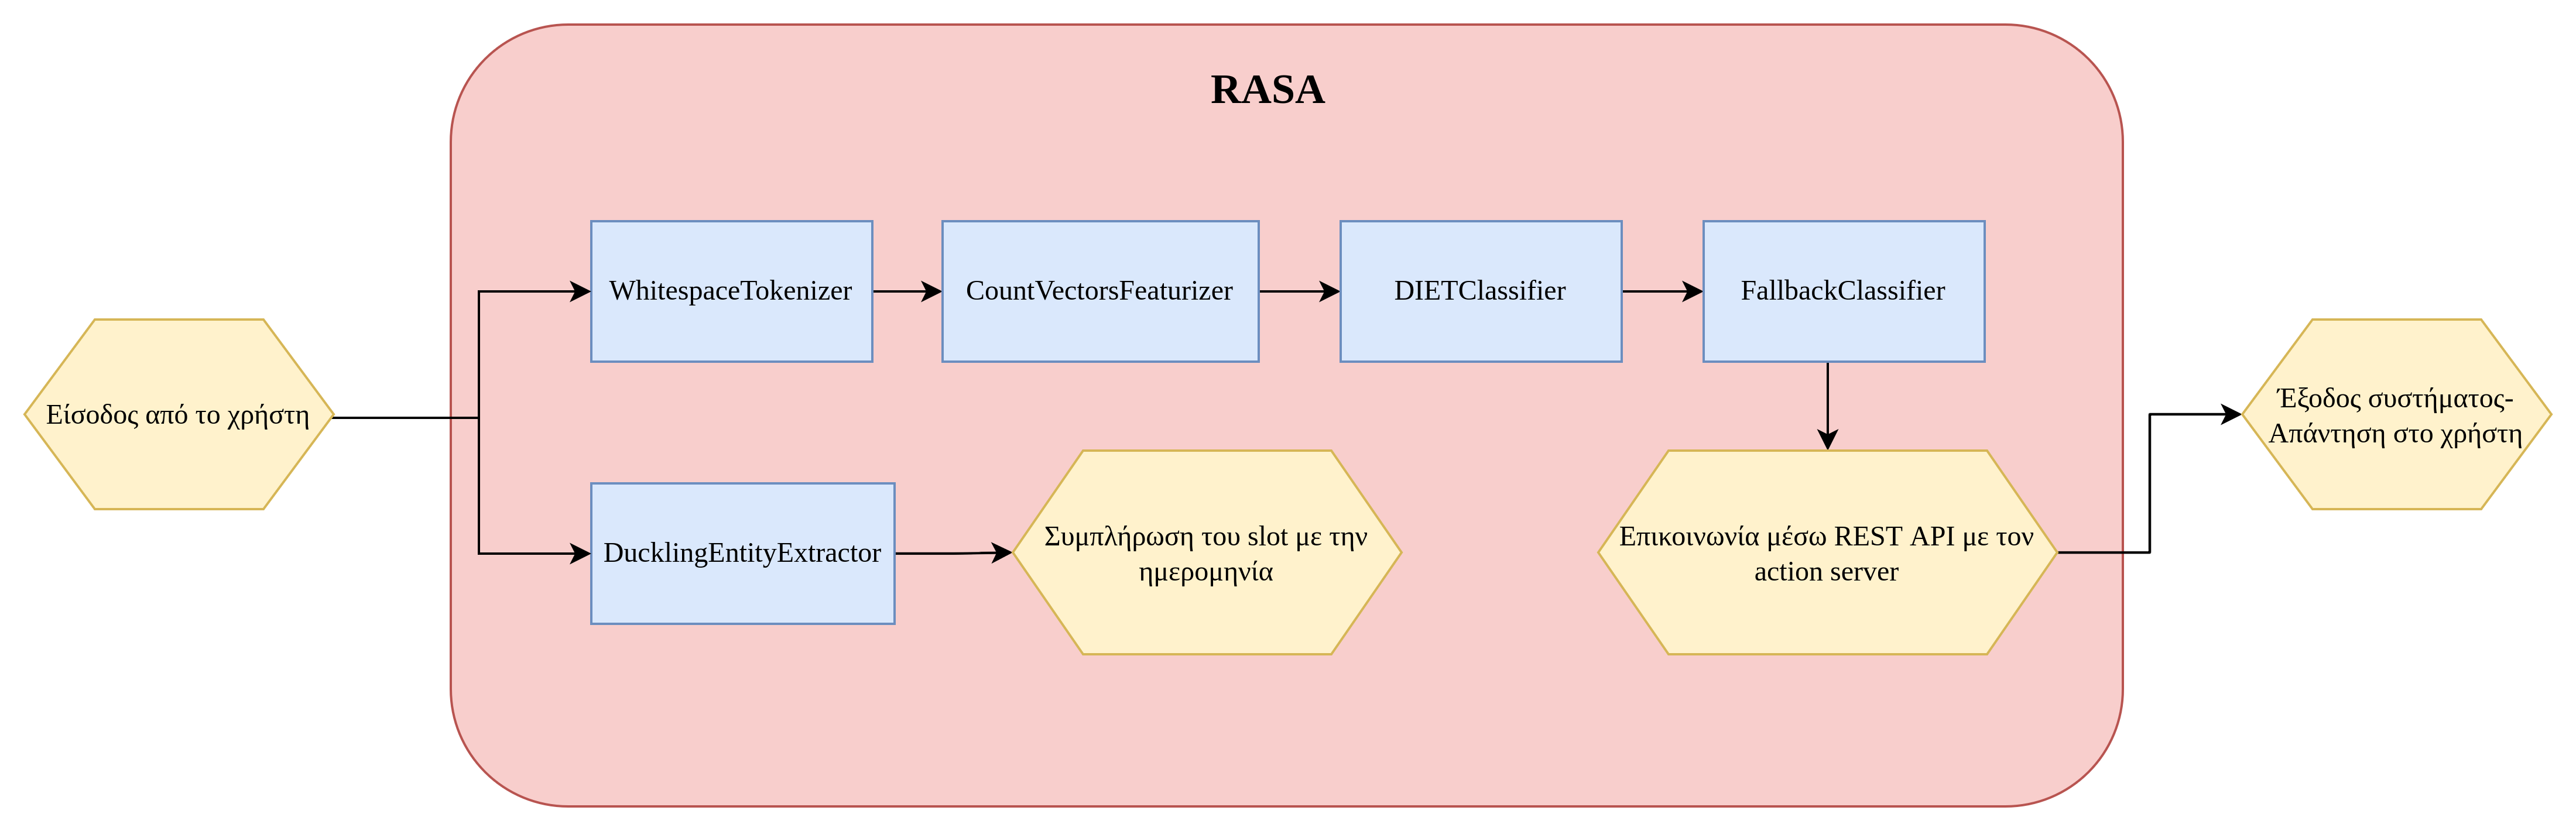
\includegraphics[width=1\textwidth]{images/chapter4/rasa.png}
  \caption{Rasa Pipeline}
  \label{fig:rasa-pipeline}
\end{figure}
\noindent

\subsubsection{\emph{WhitespaceTokenizer}}
Ως αρχικό βήμα της επεξεργασίας του μηνύματος είναι η παραγωγή των \emph{tokens}. Στη παρούσα περίπτωση χρησιμοποιείται η παραγωγή \emph{token} ανά λέξη, δηλαδή κάθε λέξη που χωρίζεται με κενό χαρακτήρα από τις υπόλοιπες αποτελεί ένα \emph{token}.

\subsubsection{\emph{CountVectorsFeaturizer}}
Από τα \emph{tokens} που έχουν παραχθεί από τον \emph{Tokenizer} ο \emph{CountVectorsFeaturizer} παράγει χαρακτηριστικά (\emph{features}) για την ταξινόμηση της επιθυμίας του χρήστη και την επιλογή της απάντησης του ψηφιακού βοηθού. Τα \emph{features} παράγονται με την μέθοδο \emph{bag-of-words}.

\subsubsection{\emph{DIETClassifier}}
Ο \emph{Dual Intent and Entity Transformer Classifier} (\emph{DIETClassifier}) χρησιμοποιείται για την εξαγωγή της επιθυμίας του χρήστη αλλά και την αναγνώριση οντοτήτων. Η αρχιτεκτονική του είναι βασισμένη στα \emph{transformers} και είναι κοινή και για τις δύο λειτουργίες. Ως είσοδος στον ταξινομητή εισέρχονται τα χαρακτηριστηκά (\emph{features}) που έχουν εξαχθεί από τον προηγούμενο κόμβο. Επιπλέον, για τη παρούσα υλοποίηση ο \emph{DIETClassifier} χρησιμοποιείται μόνο για την εξαγωγή της επιθυμίας του χρήστη.

\subsubsection{\emph{FallbackClassifier}}
Η επιθυμία του χρήστη προβλέπεται από τον \emph{DIETClassifier}. Αυτός αποδίδει ένα σκορ (μία πιθανότητα) για κάθε μία από τις διαθέσιμες επιθυμίες χρήστη. Σε περίπτωση που το σκορ είναι πιο χαμηλά από κάποιο κατώφλι (το κατώφλι τίθεται ως παράμετρος του συστήματος) ή η διαφορά των σκορ των δύο πιο πιθανών κατηγοριών είναι μικρότερη από ένα δεύτερο κατώφλι (και αυτό τίθεται ως παράμετρος του συστήματος), τότε αλλάζει την πρόβλεψη του \emph{DIETClassifier} σε \emph{nlu\_fallback}, μία ειδική κατηγορία ταξινόμησης που σηματοδοτεί την αβεβαιότητα της πρόβλεψης. Στη περίπτωση αυτή, ο ψηφιακός βοηθός ζητά από το χρήστη να αναδιατυπώσει για την εκ νέου ταξινόμηση της επιθυμίας του.

\subsubsection{\emph{DucklingEntityExtractor}}
Το \emph{Duckling} χρησιμοποιείται για την εξαγωγή οντοτήτων όπως ημερομηνίες, χρηματικά ποσά, αποστάσεις και άλλα. Στη συγκεκριμένη υλοποίηση το \emph{Duckling} χρησιμοποιείται για την εξαγωγή ημερομηνίας, σε περίπτωση που ο χρήστης επιθυμεί την αναζήτηση από συγκεκριμένη ημερομηνία και έπειτα. Η πληροφορία αυτή αποθηκεύεται σε θέσεις μνήμης που παρέχει το \emph{RASA} οι οποίες ονομάζονται \emph{slots} οι οποίες είναι διαθέσιμες και στον \emph{RASA Action Server} για την περαιτέρω επεξεργασία. 

\subsubsection{\emph{MemoizationPolicy}}
Ένα ακόμα αρχείο που παρέχεται για την εκπαίδευση του βοηθού είναι το αρχείο που περιέχει ιστορίες με πιθανά μονοπάτια συζητήσεων χρήστη-βοηθού. Αυτές οι ιστορίες βρίσκονται στο αρχείο \emph{stories.yml}, \autoref{fig:rasax-stories}. Η συγκεκριμένη πολιτική "θυμάται" τις ιστορίες αυτές και προσπαθεί να ανιχνεύσει αν η συζήτηση που γίνεται με τον χρήστη ταυτίζεται με κάποια από τις ιστορίες εκπαίδευσης. Σε περίπτωση που συμβαίνει αυτό τότε εκτελούνται τα αντίστοιχα \emph{actions} από τον βοηθό.

\subsubsection{\emph{RulePolicy}}
Η πολιτική κανόνων, όπως είναι φανερό και από το όνομα της, χειρίζεται κομμάτια συζητήσεων που ακολουθούν συγκεκριμένη συμπεριφορά. Πιο συγκεκριμένα, καθορίζει την επόμενη ενέργεια του βοηθού, βασιζόμενη στην επιθυμία του χρήστη, με βάση σύνολο κανόνων που βρίσκονται στο αρχείο \emph{rules.yml}, \autoref{fig:rasax-rules}. Για παράδειγμα όταν ανιχνεύεται ότι ο χρήστης επιθυμεί να αποχαιρετήσει τον ψηφιακό βοηθό τότε ο ίδιος πρέπει να αποχαιρετήσει το χρήστη, ανεξάρτητα από τις προηγούμενες εισόδους στη συζήτηση.

\subsubsection{\emph{TEDPolicy}}
Η πολιτική Transformer Embedding Dialogue \cite{TEDPOLICY} (TED) μπορεί να χρησιμοποιηθεί για ανίχνευση της επόμενης ενέργειας αλλά και για αναγνώριση οντοτήτων. Όπως και στον \emph{DIETClassifier}, η αρχιτεκτονική του είναι βασισμένη σε μία σειρά από κωδικοποιητές  \emph{transformer} οι οποίοι είναι κοινοί και για τις δύο λειτουργίες της. Για την πρόβλεψη της επόμενης ενέργειας η έξοδος του \emph{transformer} διαλόγου και οι ετικέτες ταξινόμησης ενέργειας συγχωνεύονται σε έναν σημασιολογικά διανυσματικό χώρο. Για την ομοιότητα με την επιθυμητή ενέργεια χρησιμοποιείται το εσωτερικό γινόμενο τον διανυσμάτων.

\subsubsection{\emph{UnexpecTEDIntentPolicy}}
Η πολιτική \emph{UnexpecTEDIntentPolicy} βοηθά στην αξιολόγηση των συζητήσεων του χρήστη με τον βοηθό και επιτρέπει την ανίχνευση μη αναμενόμενων αλλαγών στη συζήτηση. Ακολουθεί την ίδια αρχιτεκτονική με την \emph{TEDPolicy} έχοντας ωστόσο διαφορετικό στόχο. Πιο συγκεκριμένα, "μαθαίνει" το σύνολο με τις επιθυμίες χρήστη που είναι πιο πιθανό να εκδηλωθούν λαμβάνοντας υπόψιν το περιεχόμενο των συζητήσεων από τις ιστορίες που βρίσκονται στο αρχείο \emph{stories.yml}. Αξίζει να σημειωθεί ότι η συγκεκριμένη πολιτική βρίσκεται σε πειραματικό στάδιο και χρησιμοποιείται ως βοηθητική μαζί με την \emph{TEDPolicy}.

Σε περίπτωση που οι πολιτικές προβλέψουν την επιθυμία του χρήστη με ίδιο σκορ τότε η προτεραιότητα τους ορίζεται ως εξής (μεγαλύτερος αριθμός συνεπάγεται μεταλύτερη προτεραιότητα):
\begin{itemize}
    \item 6 - \emph{RulePolicy}
    \item 3 - \emph{MemoizationPolicy}
    \item 2 - \emph{UnexpecTEDIntentPolicy}
    \item 1 - \emph{TEDPolicy}
\end{itemize}